\section{Die Eulersche Zahl in der Analysis} Die Exponentialfunktion von $e$ ist möglicherweise die wichtigste Funktion der Mathematik - aus dem einfachen Grund, dass sie ihre eigene Ableitung ist. Infakt wird die Eulerische Zahl mit dieser Eigenschaft definiert, ähnlich wie $\pi$ durch den Vergleich von Umfang und Radius in einem Kreis definiert wird.
\subsection{Die Eigenschaften von $e^x$}
Wie bereits erwähnt, ist die Funtion $e^x$ ihre eigene Ableitung. Aus dieser Eigenschaft lassen sich gleich 2 bekannte Formeln für das Berechnen von $e$ herleiten:
\subsubsection{Die Eulersche Zahl als undendliche Summation}
\[e^x = \sum_{n=0}^\infty \frac{x^n}{n!}
  \]Um dies zu beweisen, kann die Ableitungseigenschaft genutzt werden. Da die Exponentialfunktion ihre eigene Ableitung ist, müsste dies daher auch für die Summation gelten.  \[
  \sum_{n=0}^\infty \frac{x^n}{n!} = \frac{d}{dx}\sum_{n=0}^\infty \frac{x^n}{n!} = \sum_{n=0}^\infty \frac{d}{dx}\frac{x^n}{n!} 
  \] Dank der Summationsregel von Ableitungen kann man die Ableitung auf jeden Summanten einzeln anwenden. Schreibt man diese Summe dann aus, dann wird es schnell eindeutig, dass die Funktion sich nicht verändert hat. \[
  \sum_{n=0}^\infty \frac{x^n}{n!} = 1 + \frac{x}{1} + \frac{x^2}{2} + \frac{x^3}{6} + \frac{x^4}{24} + \frac{x^5}{120} + \dots
  \] \[
  \sum_{n=0}^\infty \frac{d}{dx}\frac{x^{n}}{n!} = 0 +  1 + \frac{x}{1} + \frac{x^2}{2} + \frac{x^3}{6} + \frac{x^4}{24} + \dots
\]Weil die Gleichheit der 2 Terme dadurch bewiesen ist, kann man nun durch das Einsetzen von x durch 1 die Eulerische Zahl mithilfe der Summation berechnen. \[
  \begin{aligned}
    \frac{1}{0!} + \frac{1}{1!} = \indent\crel{2},\underline{0}\\
    \frac{1}{0!} + \frac{1}{1!} + \dots + \frac{1}{10!} =  \indent\crel{2},7182818\underline{0}\dots\\
    \frac{1}{0!} + \frac{1}{1!} + \dots + \frac{1}{100!} = \indent\crel{2},718281828459\dots
  \end{aligned}
\] \newpage
Wenn bis n = 1 gerechnet wird, stimmt keine Kommastelle überein. Rechnet man bis 10, dann stimmen die ersten 7 Kommastellen mit der tatsächlichen Zahl überein. Beim Ausrechnen bis n = 100 sind bereits die ersten 159 Stellen richtig. Insgessamt scheint mir diese Näherung daher als mögliche Option für das Berechnen von $e$ auf 100.000 Nachkommastellen.
\begin{figure}[h]
  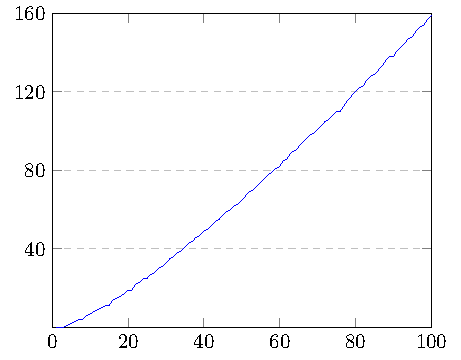
\includegraphics{medien2/summation/summation.pdf}
  \centering
\end{figure}
\par Die X-Achse repräsentiert die Anzahl an richtigen Nachkommastellen und die Y-Achse zeigt die Anzahl an Summationen. Der Graph deutet dabei auf lineares Wachstum hin.
\subsubsection{Die Eulersche Zahl als Limes}
Die zweite Formel für $e$, die sich aus ihrer Ableitung herleiten lässt, kommt dann zustande, wenn man die Ableitung nach ihrer Definition betrachtet. \[
e^x = \lim_{h\to0} \frac{e^{x+h}-e^x}{h}\]
Diese Formel kann man wie folgt nach $e$ umstellen:\[
e = \lim_{h\to0} (h + 1)^{\frac{1}{h}}\] 
und $h$ wird meistens mit $\frac{1}{n}$ substituiert, um die Formel zu vereinfachen.\[
e = \lim_{n\to\infty} (1+\frac{1}{n})^n\]
Berechnet man $e$ mit dieser Formel, dann erhält man die folgenden Werte: \[
  \begin{aligned}
  (1+\frac{1}{1})^1 = \indent\crel{2},\underline{0}\\
  (1+\frac{1}{10})^{10} =  \indent\crel{2},\underline{5}\dots\\
  (1+\frac{1}{100})^{100} = \indent\crel{2},7\underline{0}\dots
\end{aligned} \]
Die Konvergenz zum tatsächlichen Wert ist hierbei unglaublich langsam im Vergleich zu der voherigen Summation, was mich sehr überrascht hat, denn beide Formeln wurden ja aus der gleichen Eigenschaft gewonnen.
\begin{figure}[h]
  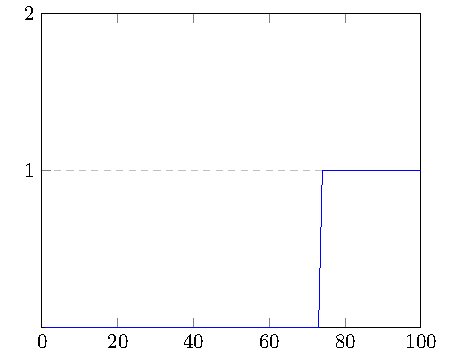
\includegraphics{medien2/limes/limes.pdf}
  \centering
\end{figure}
